\section{Controller design process}

\subsection{Failed design approaches}

Several attempts were made using a variety of methods before a working controller was developed. One of the primary mistakes was using SIMULINK's model linearisation tool to build a transfer function from the plant. Certain elements of the plant cannot be linearised and doing this process produced a plant with purely imaginary zeroes. The plant poles produced by this method however, were mostly correct. SIMULINK's output included 3 poles at the origin, as well as at around -535 and -80. This approach was dumped and the correct plant transfer function was built using Mason's Gain Formula on the plant signal flow graph provided.

From this new transfer function, a few design approaches were tried, one was using the linear algebraic method in an attempt to create a two-degrees of freedom controller. However, LAMdesign cannot deal with the amount of poles at the origin in this plant, and simply will not give any usable output. This left only the unity feedback controller available as an option, as the system was going to have to be designed using the outward approach.

After obtaining the new plant transfer function, we attempted to use MATLAB's sisotool in order to design a controller. Sisotool allows the user to place the poles and zeros of the controller directly on the root locus plot or Bode diagram. Sisotool gave us some problems, that were later solved during design using standard root locus techniques.


\subsection{Root Locus Design}

The final design was a unity feedback, 4 term controller. Poles and zeros were placed in the transfer function and moved around in order to get the root locus plot "in the ballpark" of minimal overshoot and minimum response time. Problems arose when attempting to do this because the transfer function of the plant was initially negative and the gain used in the first couple of controller designs was positive. Switching to a negative gain fixed this problem and resulted in the root locus behaviour becoming as expected. Best results were achieved using 3 zeros at -1 (the minimum radial distance from plant poles) and plant poles at -5, -4 and -3.5. Moving the plant poles farther away from the j$\omega$ axis reduced both overshoot and settling time. This also had the adverse effect of rolling the ball off of the wrong side of the track once the input was given. controller poles had to be moved closer to the j$\omega$ axis for this reason. Control effort from this design was very high, and it exhibited fairly high settling time, and 1cm overshoot. The step response of this design is shown below in figure  \ref{3:fig:stepresponse} , its root locus plot is on page \pageref{2:fig:rlocus}.


\begin{figure}[h]
	\centering
		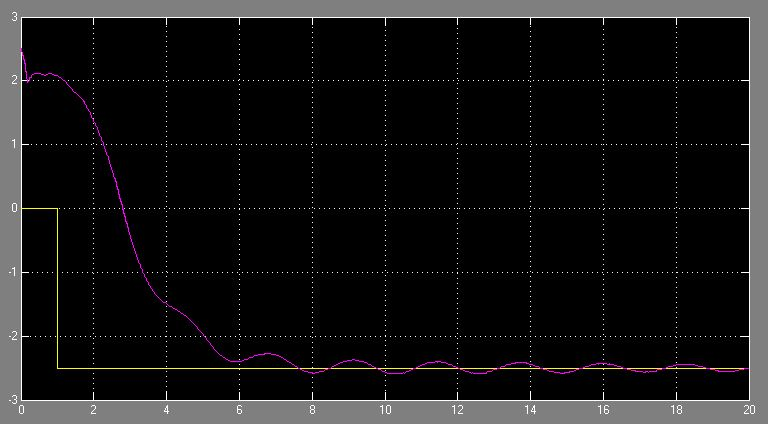
\includegraphics[width=0.70\textwidth]{pics/stepresponse}
	\caption{Root locus design step response (.1V/cm)}
	\label{3:fig:stepresponse}
\end{figure}
\begin{figure}[h]
	\centering
		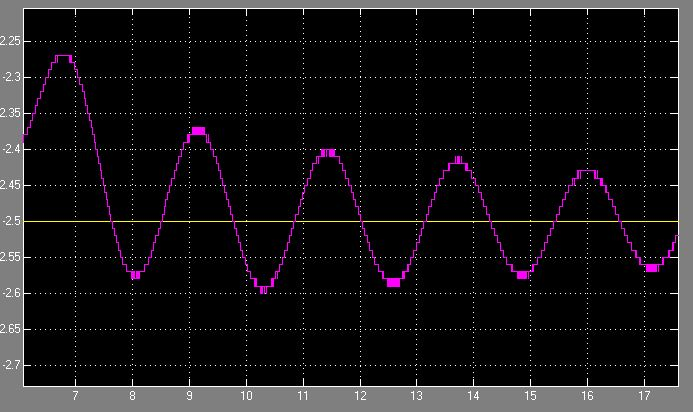
\includegraphics[width=0.70\textwidth]{pics/maximumovershoot}
	\caption{Root locus design maximum overshoot (.1V/cm)}
	\label{3:fig:maximumovershoot}
\end{figure}
\FloatBarrier

Overshoot is a maximum of 1cm occuring at approximately 10.25 seconds. Control effort is fairly high throughout the range, but the graph shows how it reduces as the ball settles out on the track.

\begin{figure}[h]
	\centering
		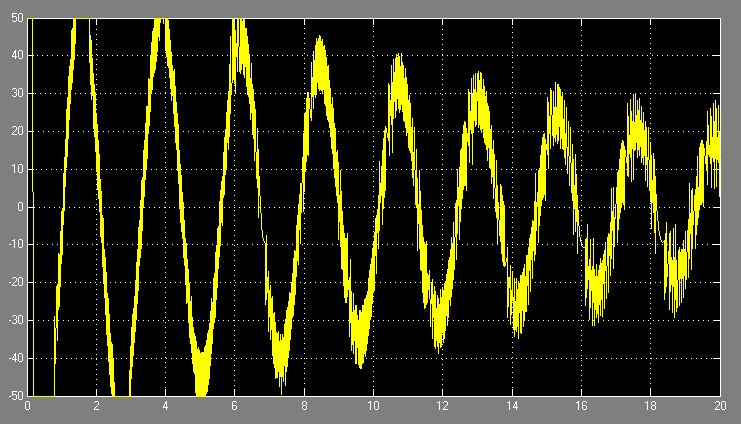
\includegraphics[width=0.70\textwidth]{pics/controleffort}
	\caption{Root locus design control effort (50V limited)}
	\label{3:fig:controleffort}
\end{figure}
\FloatBarrier

Control effort is near maximum and stays over 50\% for 20 seconds. This is most likely due to the high amounts of overshoot in controlling this particular plant. This results in the controller "hunting" for the proper location. It is overshooting partially because the response is too slow, but that cannot be sped up without sacrificing necessary precision.

\pagebreak

\subsection{Tweaking with SISOtool}

After selecting this design (and all plant parameters including the motor and gearbox), we went back to sisotool to see if there was a way to fix the earlier problems. By setting the initial gain of the compensator to -1 instead of 1, the root locus plot behaved as intended and we were now able to perform rapid adjustments on the fly. Use of sisotool allowed us to dynamically adjust the poles and zeros of the controller with a real-time display of the open loop step response. In this way, more design ideas could be tried with instant feedback of results. These new controller parameters provided a faster step response, and cut maximum overshoot to half a centimeter. The control effort was also reduced (initial control effort is high, but falls down to less than half of maximum when the system settles out).

\begin{figure}[ht]
	\centering
		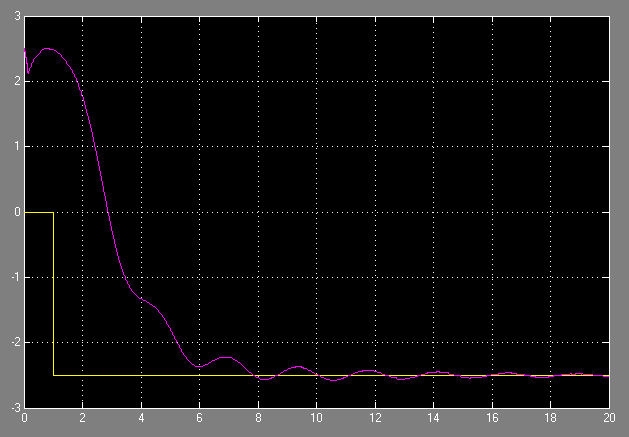
\includegraphics[width=0.70\textwidth]{pics/sisostep}
	\caption{SISO modified step response (.1V/cm)}
	\label{3:fig:sisostep}
\end{figure}

The function brings the ball to the desired location in slightly less time but the more important factor here was minimizing overshoot. The long rise time can be attributed to the input shaper, which severely damps the step input. Without this input shaper the step response would throw the ball off the wrong end of the track, so it is necessary.

\begin{figure}[ht]
	\centering
		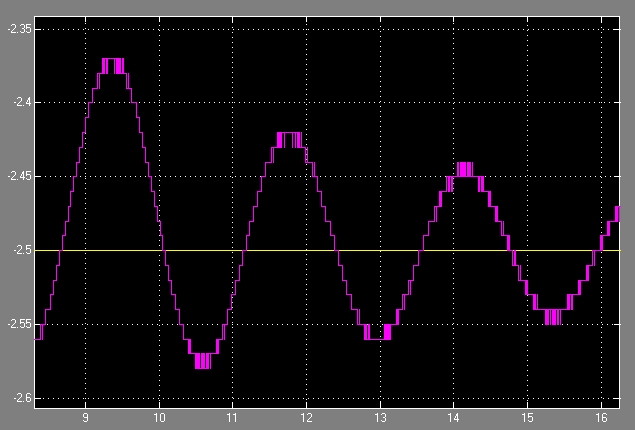
\includegraphics[width=0.70\textwidth]{pics/sisots}
	\caption{SISO modified maximum overshoot (.1V/cm)}
	\label{3:fig:sisots}
\end{figure}

The ball now settles within 1cm by 9.8 seconds. $\frac{1}{2}$cm precision comes in about 14.5 seconds. By comparison, the previous root locus design took 11.5 seconds to get to 1cm, and 20 seconds to get to $\frac{1}{2}$cm. Control effort comes down more quickly from this modified design. Compare to figure \ref{3:fig:controleffort}.

\begin{figure}[ht]
	\centering
		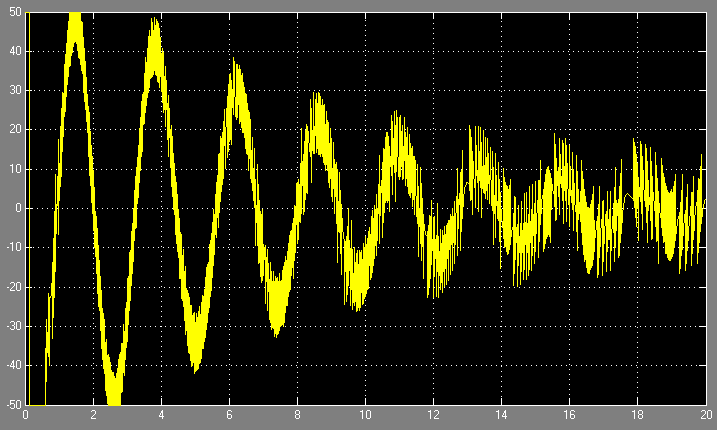
\includegraphics[width=0.70\textwidth]{pics/sisoce}
	\caption{SISO modified control effort)}
	\label{3:fig:sisoce}
\end{figure}

\clearpage